\documentclass[12pt]{article}

\usepackage{epsfig}
\begin{document}
	\pagenumbering{gobble}
	
	\begin{figure}[htp!]
		\centering
		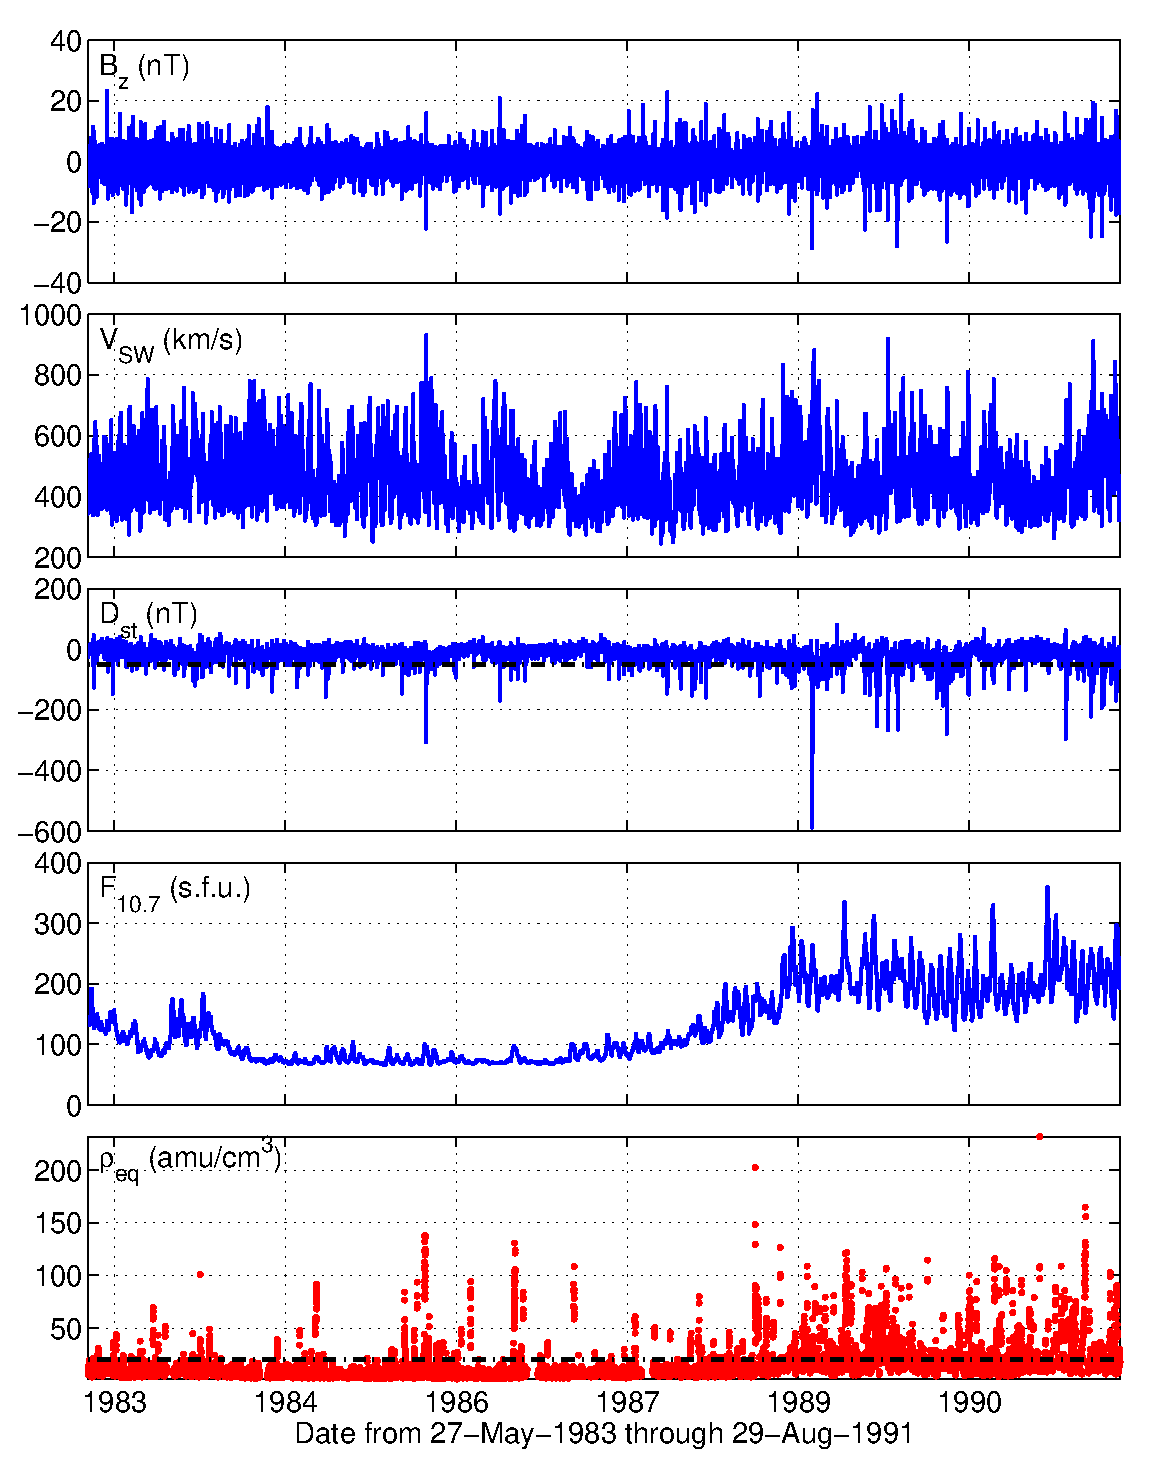
\includegraphics[scale=0.45]{2016SW001507R-p01.eps}
	\end{figure}
	
	
	
	\clearpage
	
	\begin{figure}[htp!]
		\centering
		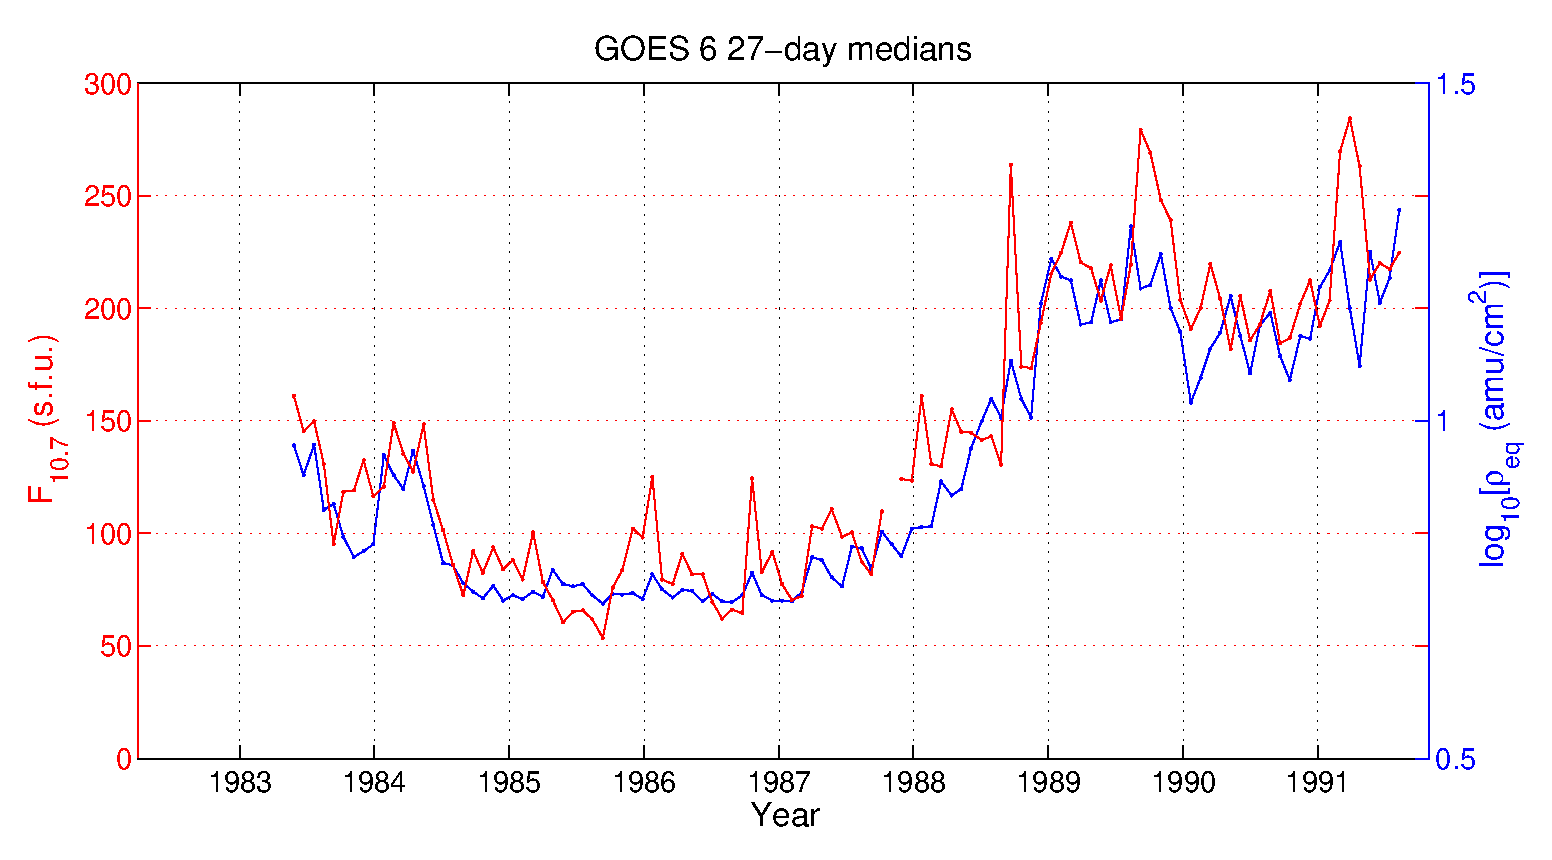
\includegraphics[scale=0.40]{2016SW001507R-p02a.eps}
		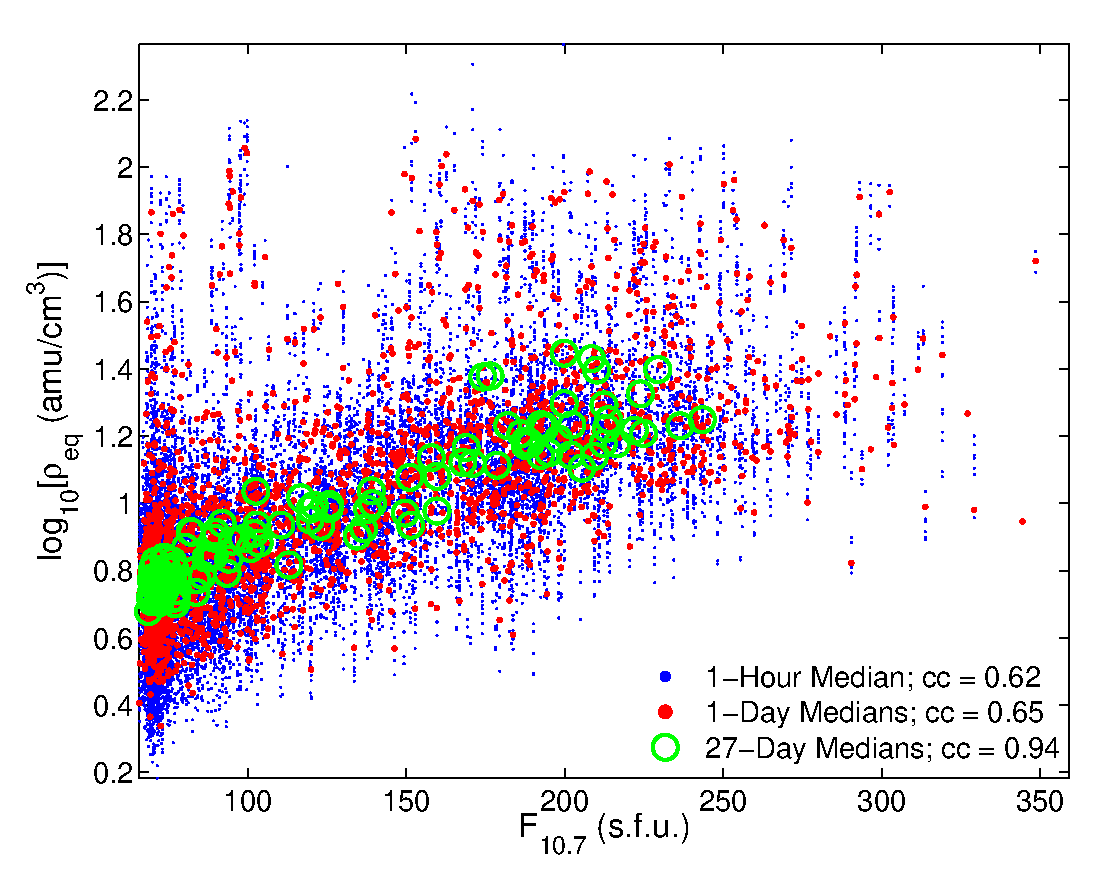
\includegraphics[scale=0.40]{2016SW001507R-p02b.eps}
	\end{figure}
	\clearpage
	
	\begin{figure}[h]
		\centering
		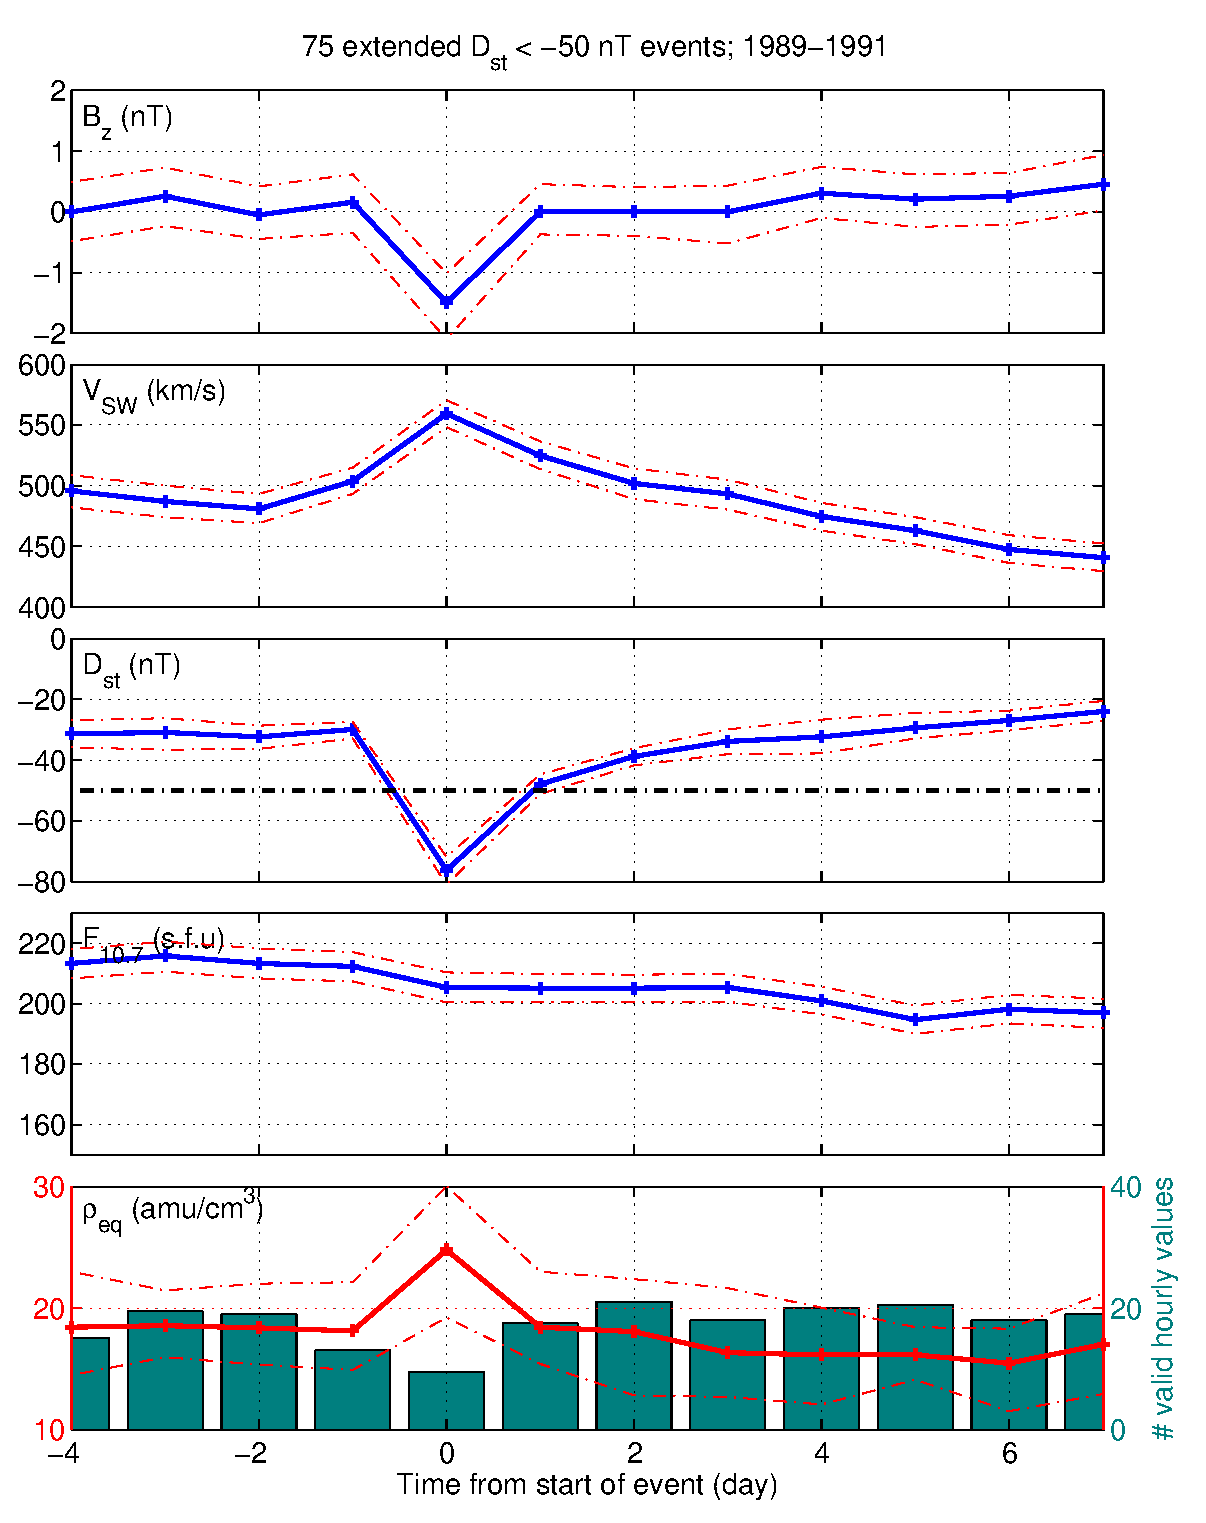
\includegraphics[scale=0.40]{2016SW001507R-p03a.eps}
		\\
		\rule[1ex]{5cm}{1pt}
		\\
		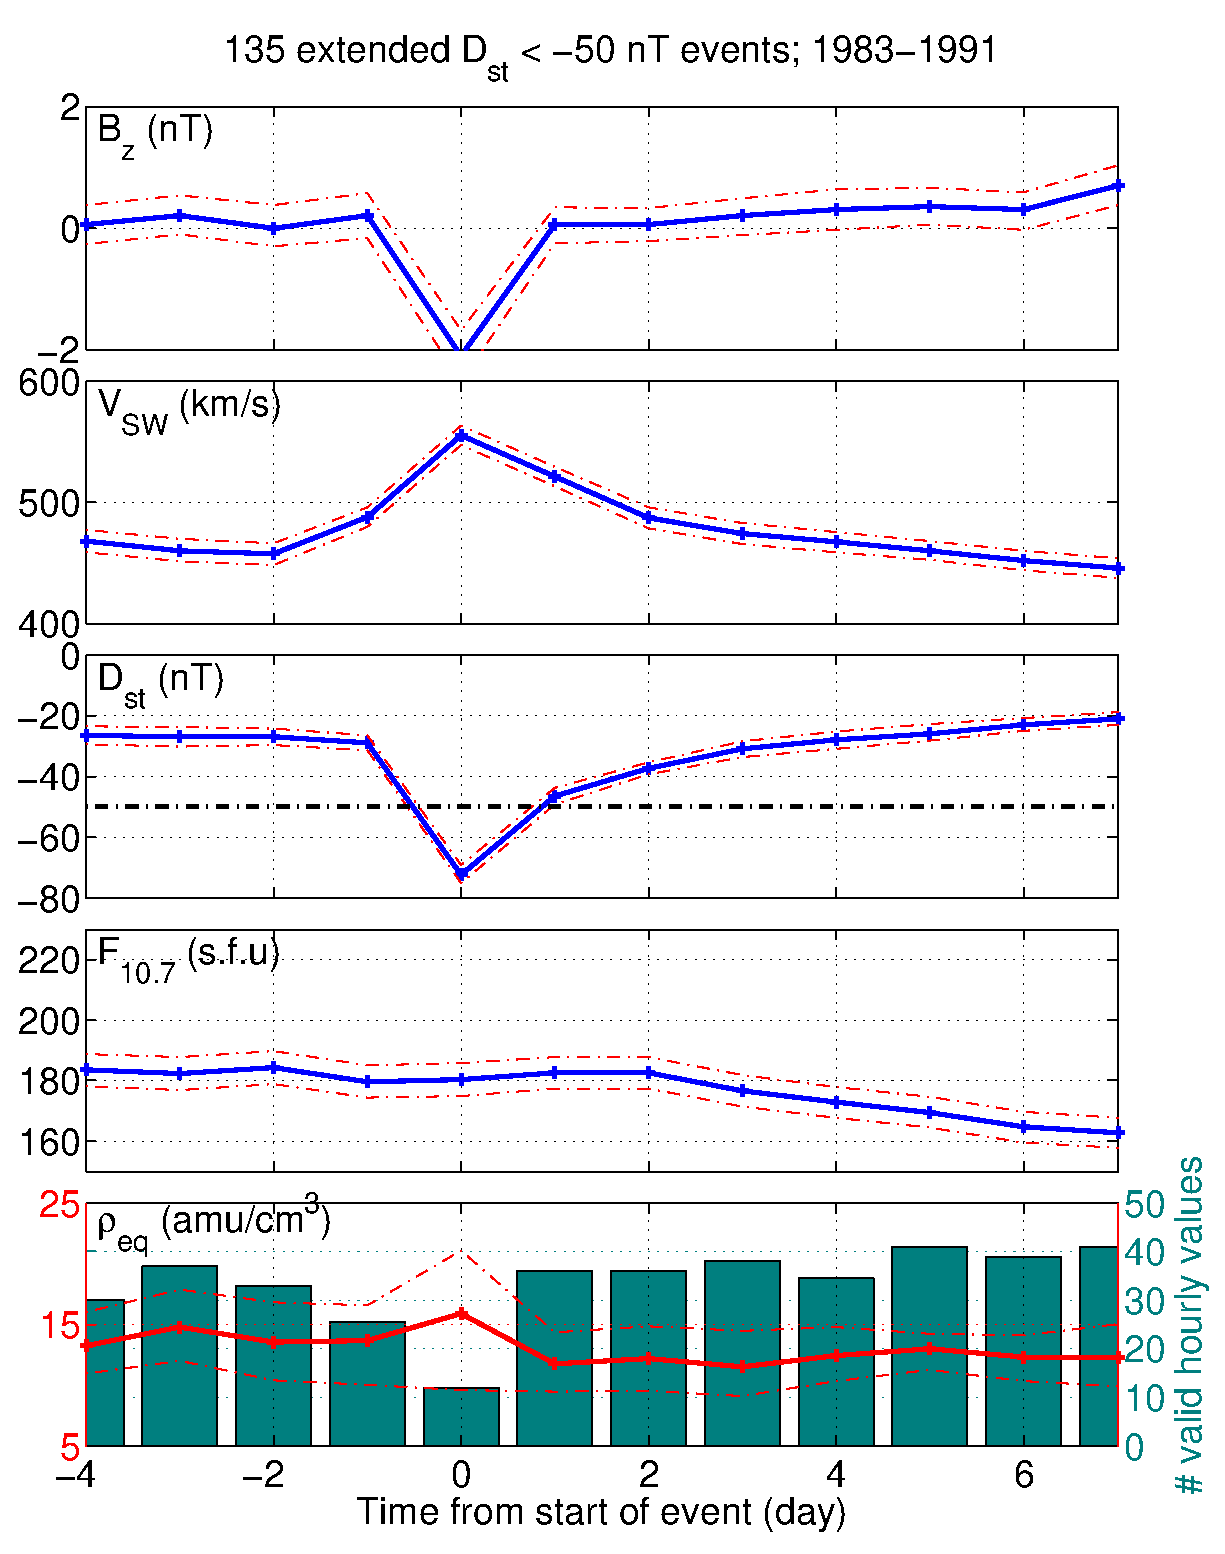
\includegraphics[scale=0.40]{2016SW001507R-p03b.eps}
	\end{figure}
	
	\clearpage
	
	\begin{figure}[tp!]
		\centering
		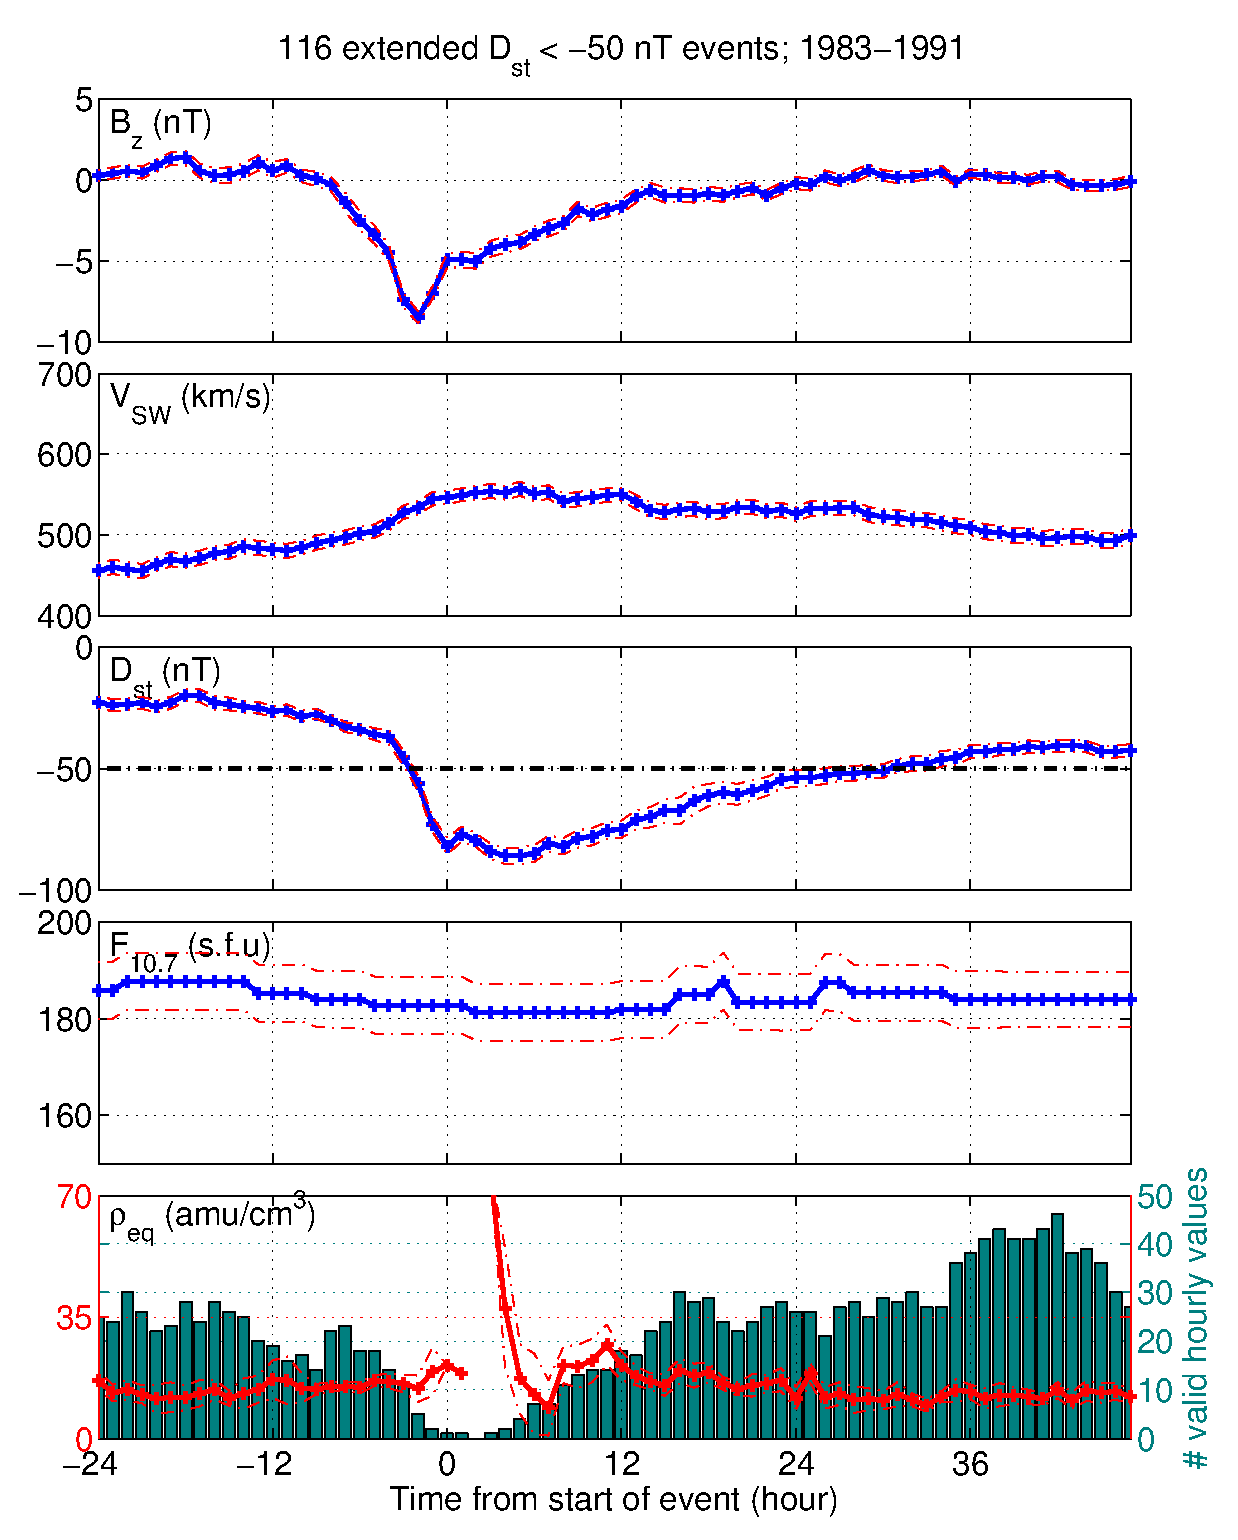
\includegraphics[scale=0.40]{2016SW001507R-p04a.eps}
		\\
		\rule[1ex]{5cm}{1pt}
		\\
		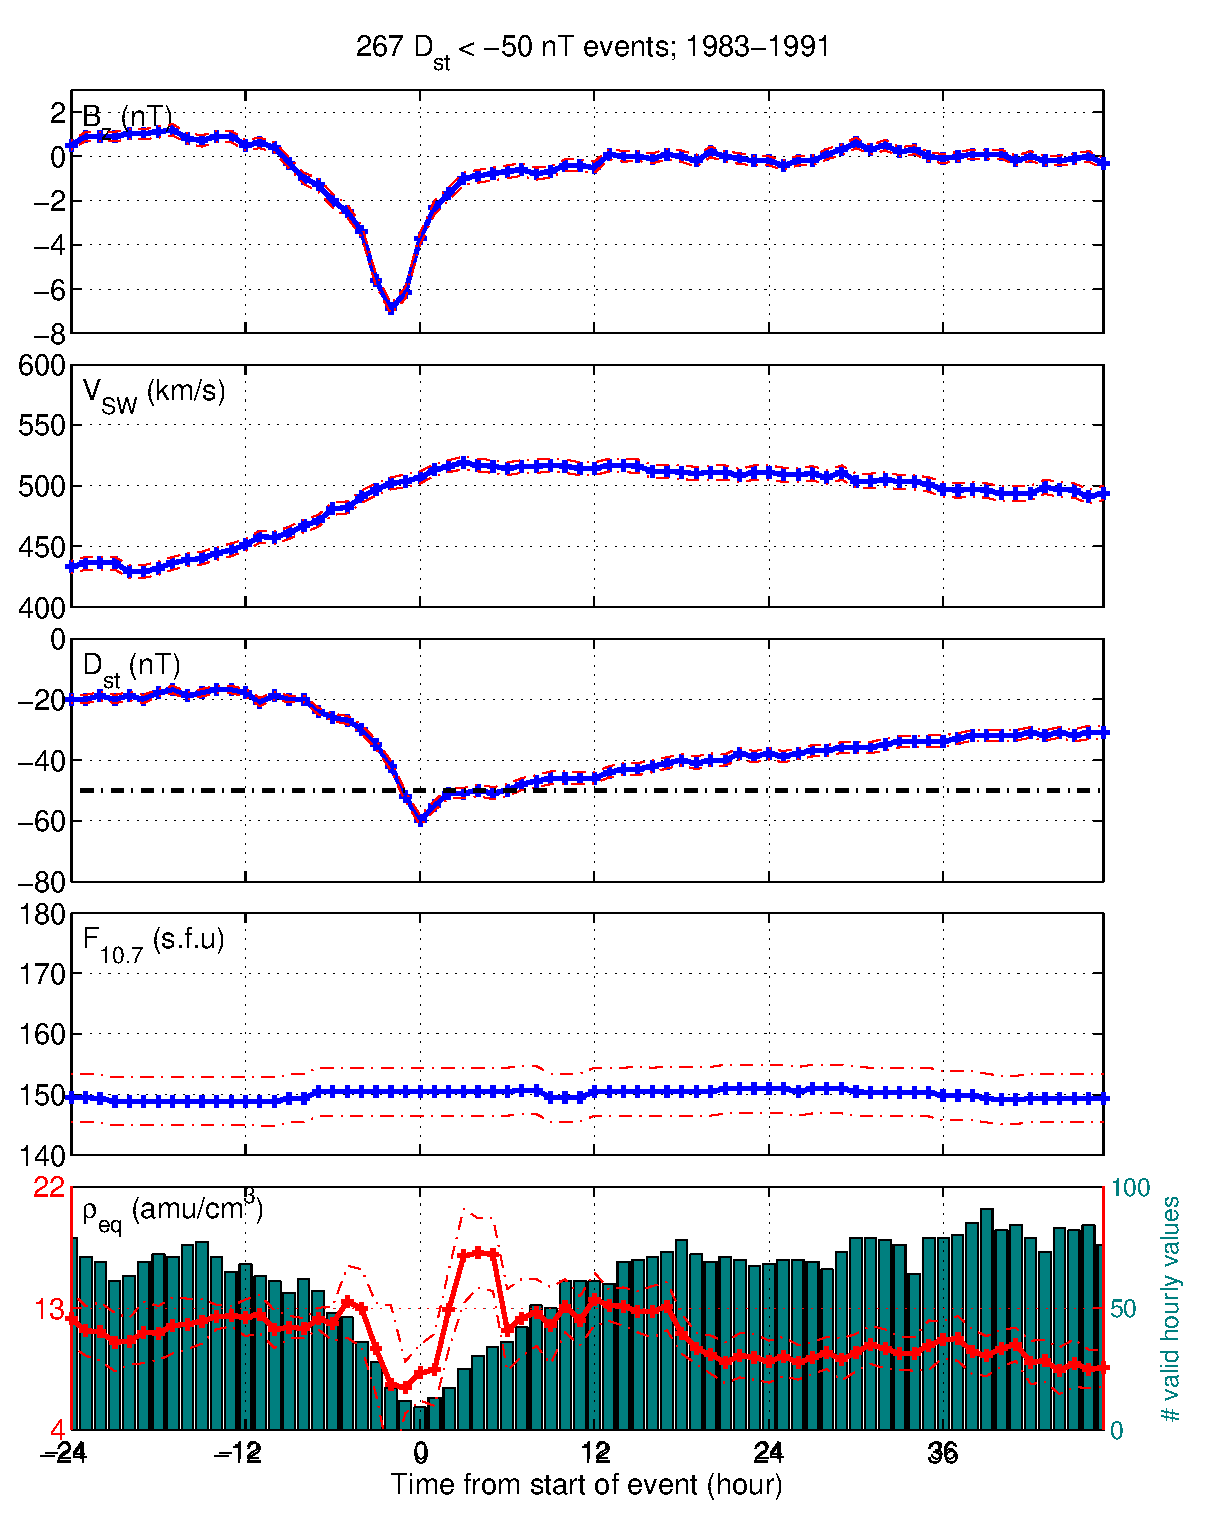
\includegraphics[scale=0.40]{2016SW001507R-p04b.eps}
		\caption{$D_{st}$ events from GOES 6 using hourly medians. Top: Events with the constraint that $D_{st}$ stayed below $-50$~nT for at least 12~hours after crossing below $-50$~nT.  Bottom: Same as Top except without constraint.}
		\label{fig:HourlyAveragedDstEvents}
	\end{figure}
	
	\clearpage
	\begin{figure}[tp!]
		\centering
		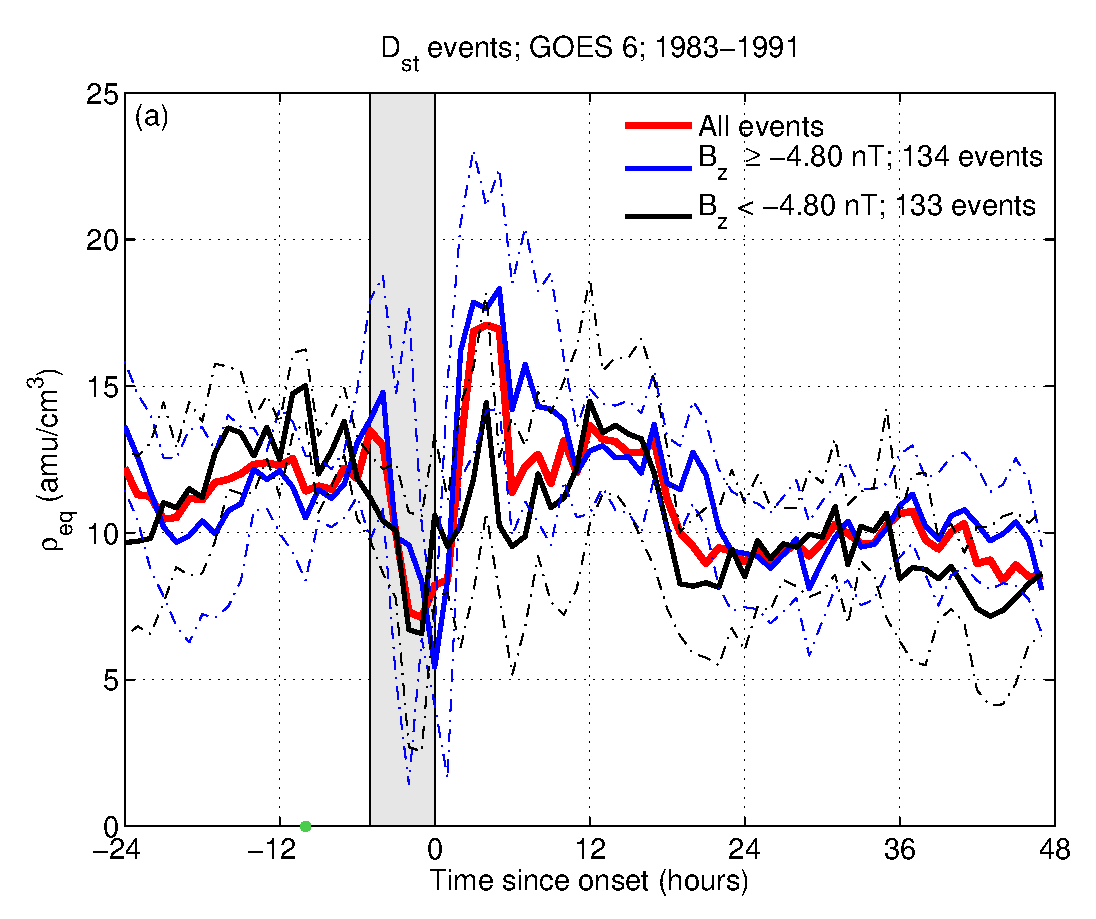
\includegraphics[scale=0.40]{2016SW001507R-p05a.eps}
		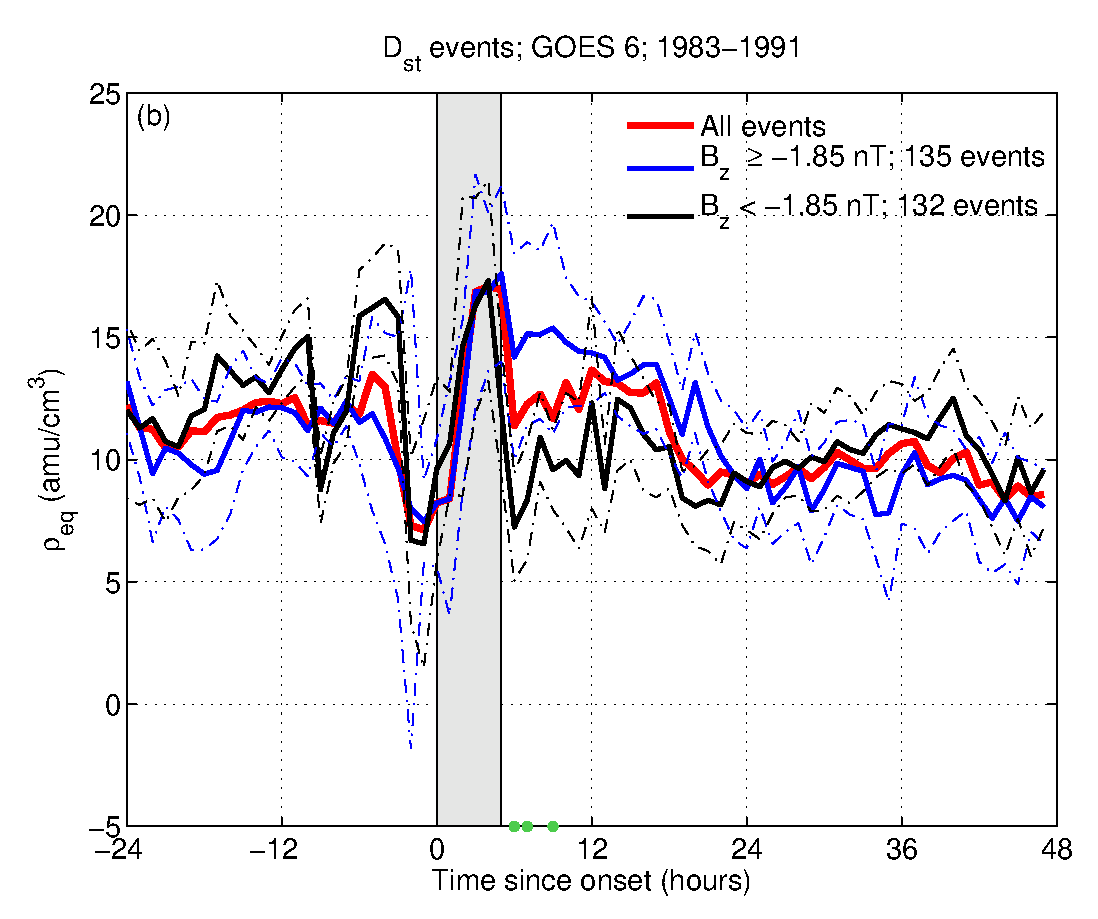
\includegraphics[scale=0.40]{2016SW001507R-p05b.eps}
	\end{figure}
	
	\begin{figure}[tp!]
		\centering
		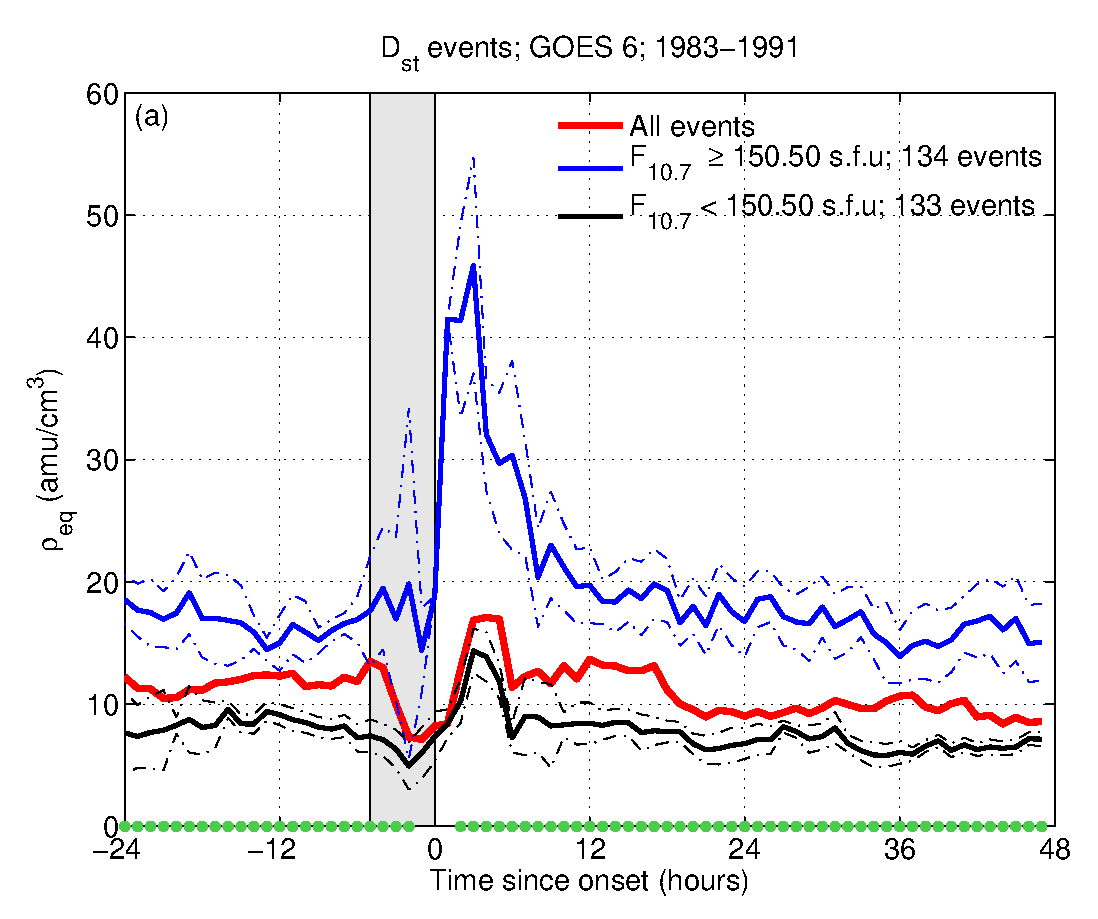
\includegraphics[scale=0.40]{2016SW001507R-p06a.eps}
		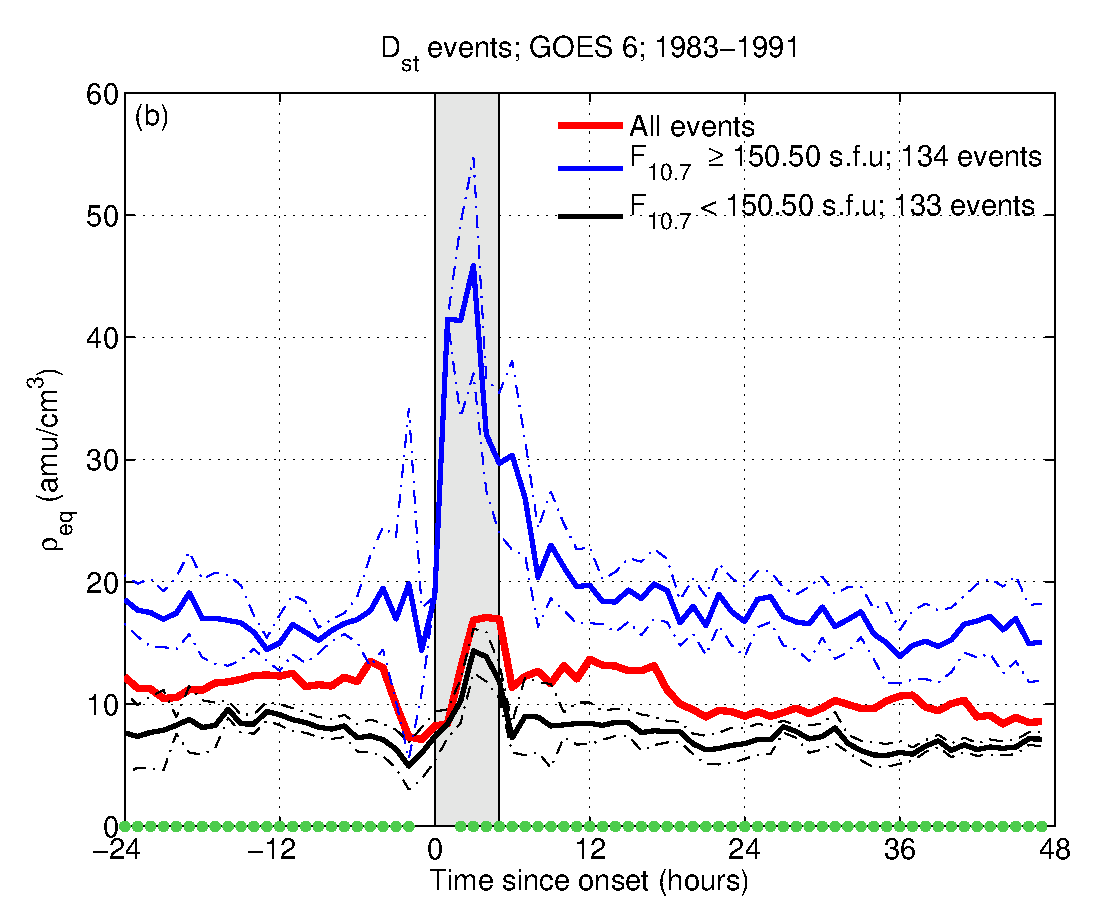
\includegraphics[scale=0.40]{2016SW001507R-p06b.eps}
	\end{figure}
	
	\clearpage
	
	\begin{figure}[htp!]
		\centering
		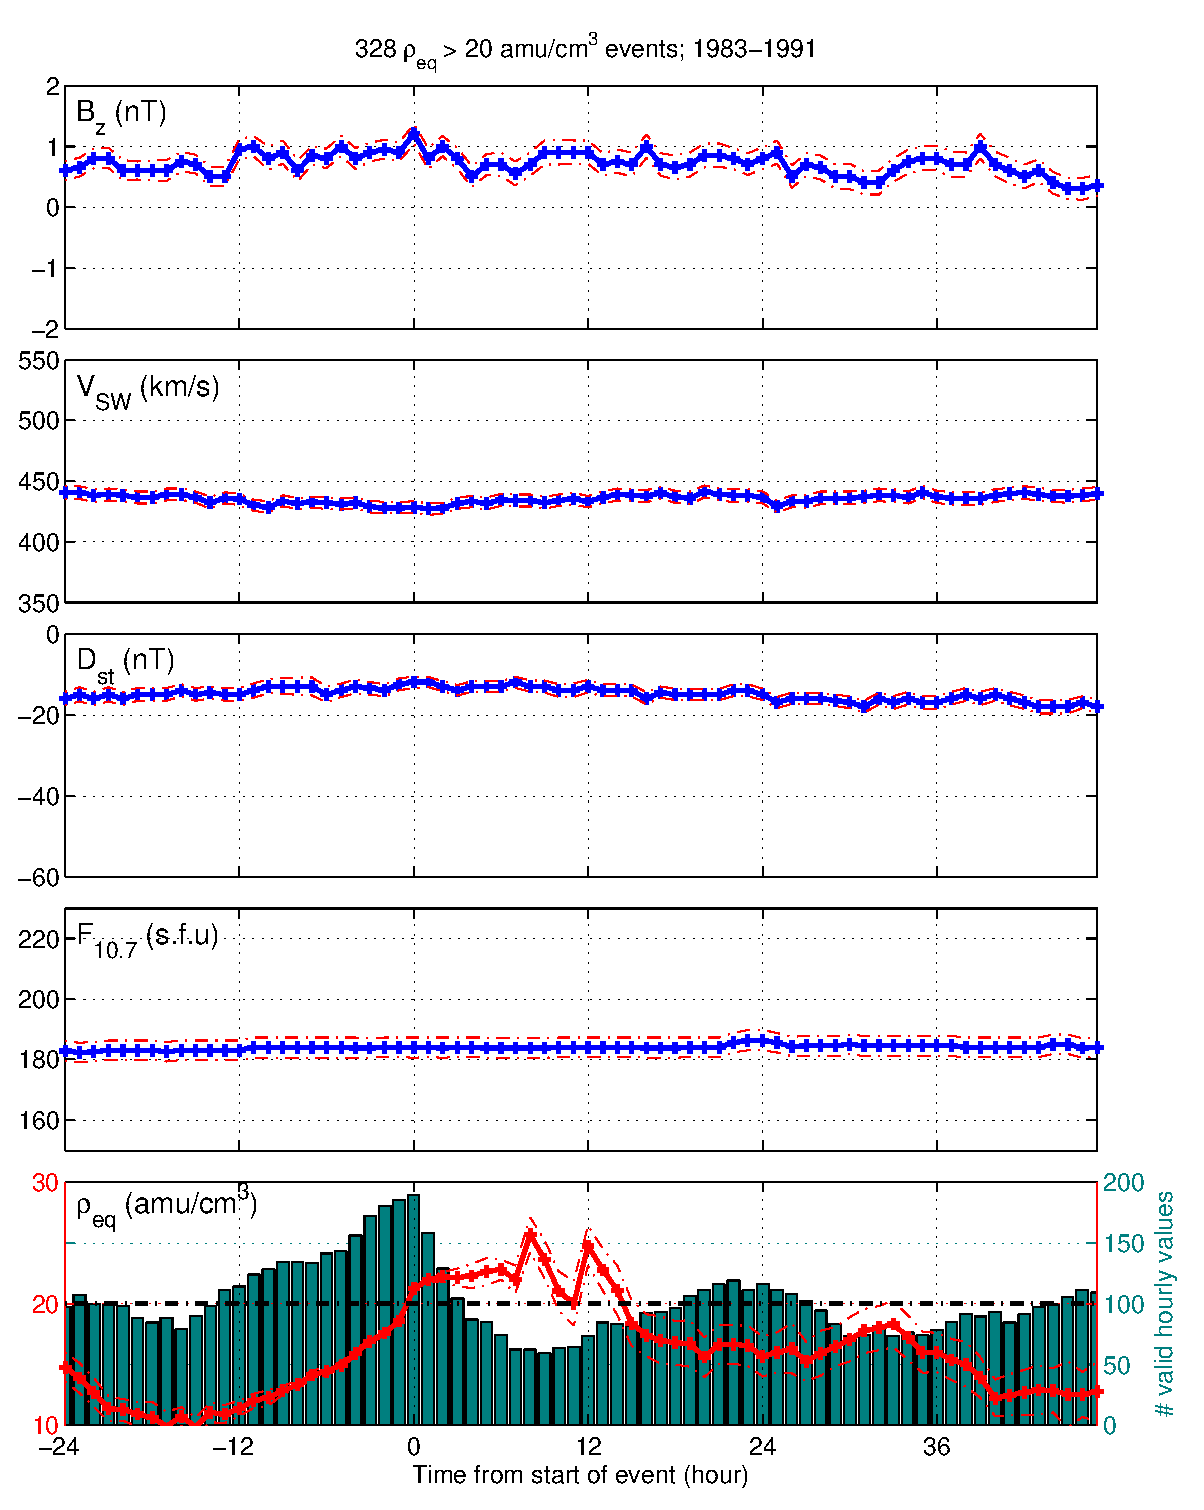
\includegraphics[scale=0.40]{2016SW001507R-p07.eps}
	\end{figure}
	
	\clearpage
	\begin{figure}[tp!]
		\centering
		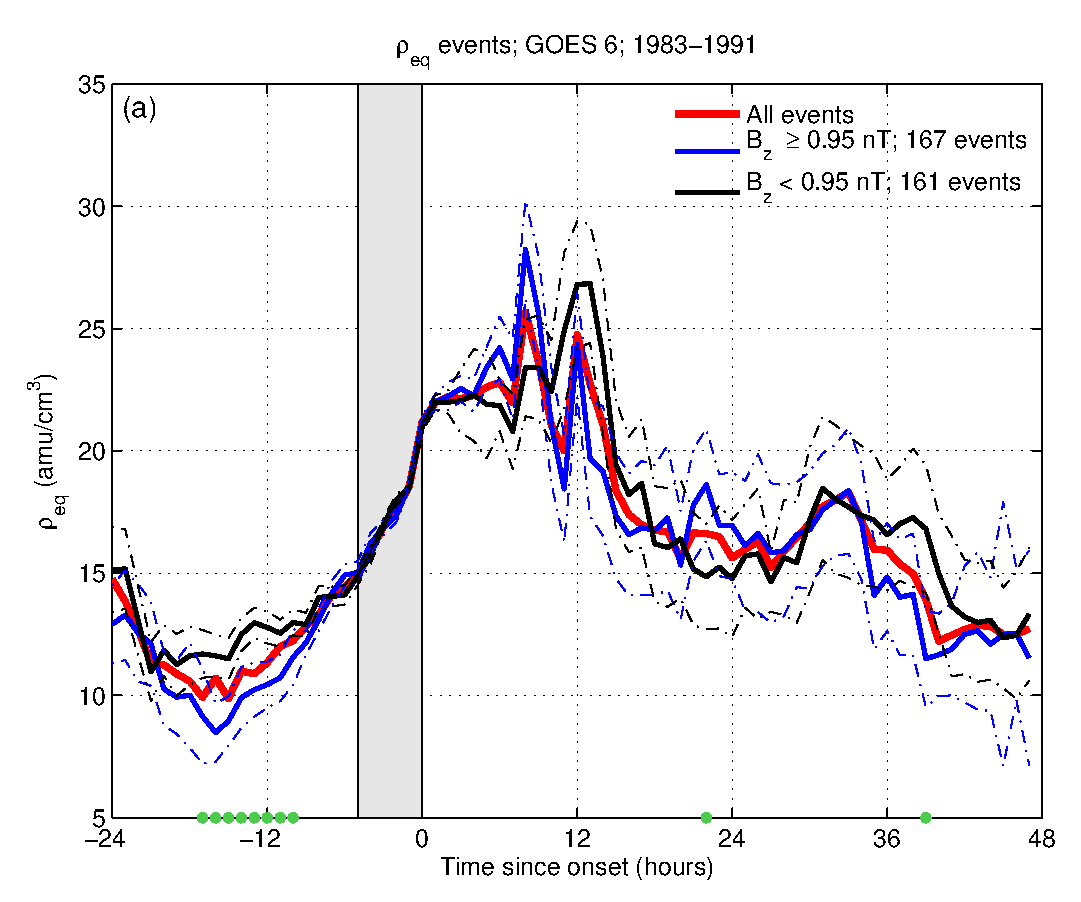
\includegraphics[scale=0.40]{2016SW001507R-p08a.eps}
		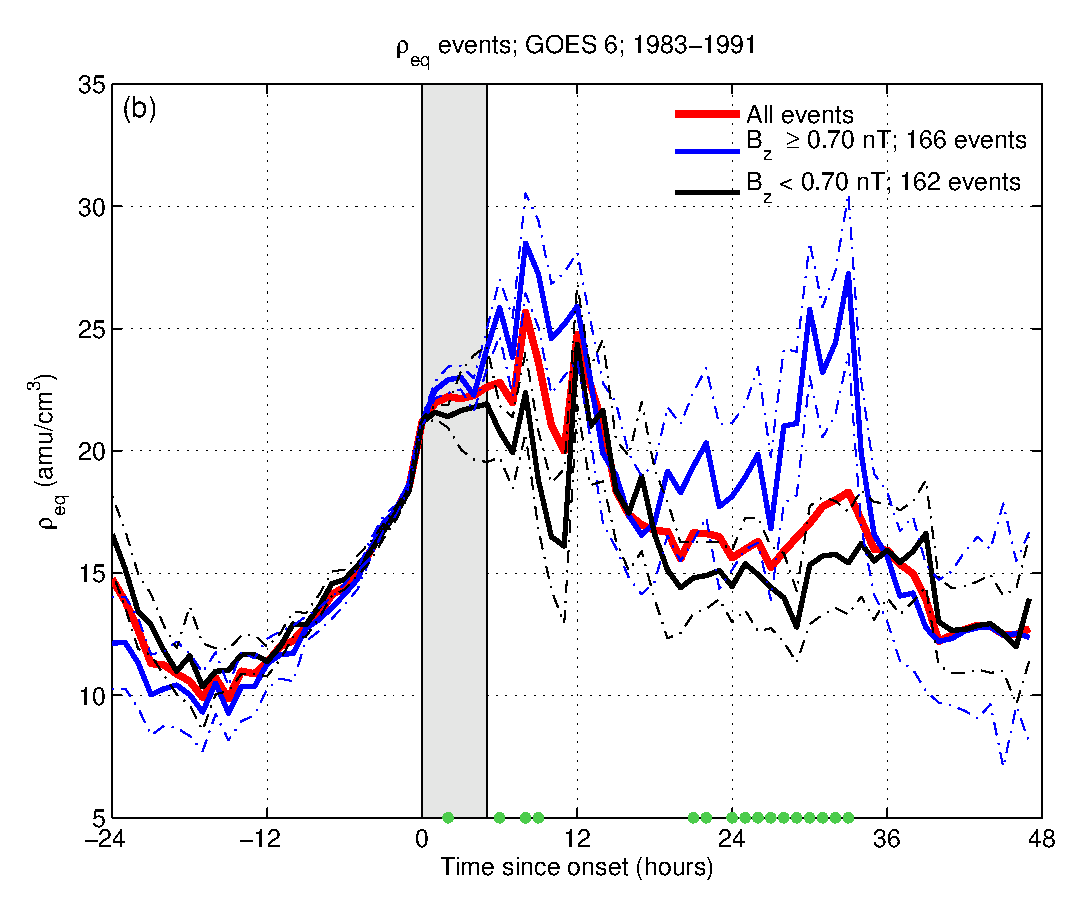
\includegraphics[scale=0.40]{2016SW001507R-p08b.eps}
	\end{figure}
	
	\begin{figure}[tp!]
		\centering
		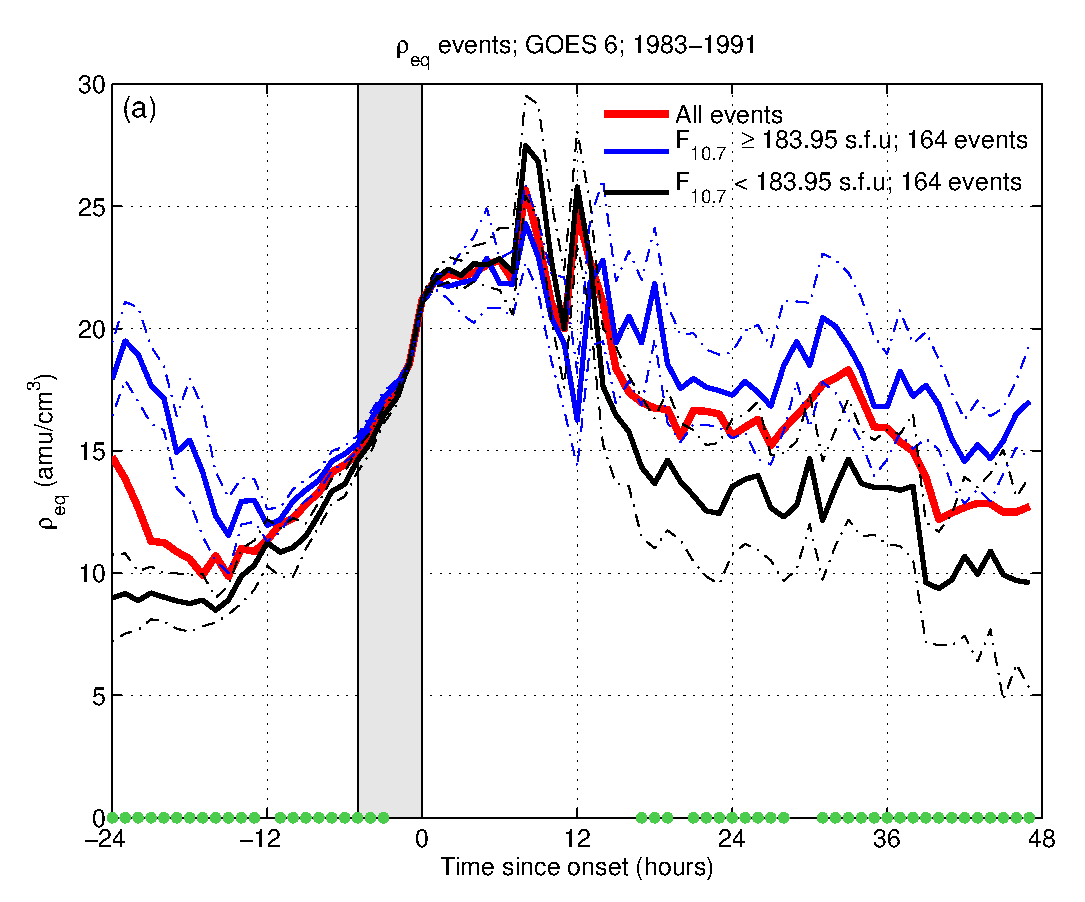
\includegraphics[scale=0.40]{2016SW001507R-p09a.eps}
		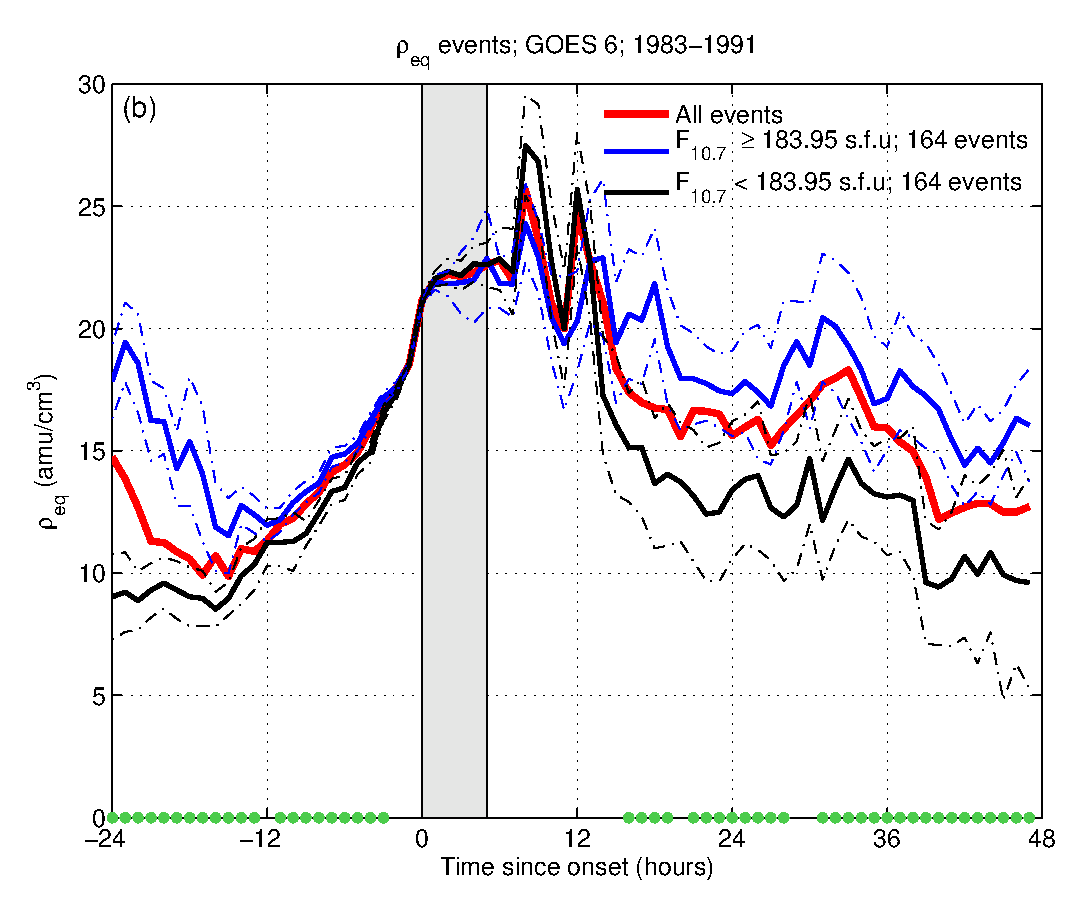
\includegraphics[scale=0.40]{2016SW001507R-p09b.eps}
	\end{figure}
	
	
\end{document}
